%COMANDO CHE DETERMINA IL TIPO DI DOCUMENTO CHE SI VUOLE CREARE

\documentclass[a4paper,12pt]{report}

%ELENCO DEI PACCHETTI UTILI PER LA STESURA DEL DOCUMENTO
\usepackage{enumitem}
\usepackage[utf8]{inputenc}
\usepackage[english, italian]{babel}
\usepackage{graphicx}
\usepackage{float}
\usepackage{tabularx}
\usepackage{makecell}
\usepackage{titlesec}
\usepackage{fancyhdr}
\usepackage{lastpage}
\usepackage{xurl}
\usepackage{hyperref}
\usepackage{geometry}
\usepackage[table,dvipsnames]{xcolor}
\setcounter{tocdepth}{5}
\setcounter{secnumdepth}{5}
\usepackage{caption}
\usepackage{etoolbox}% >= v2.1 2011-01-03
\usepackage{tikz}
\usepackage{listings}
\usepackage{scalerel}
\usepackage{longtable}
\captionsetup[table]{position=bottom}
\usepackage{comment}
\titleformat{\chapter}[display]
{\normalfont\bfseries}{}{0pt}{\LARGE}

%COMANDO PER LA SPAZIATURA DEI TITOLI DAL BORDO DEL FOGLIO

\titlespacing*{\chapter}{0cm}{0cm}{0.2cm}

%COMANDO PER LA SPAZIATURA DEL TESTO DAI BORDI LATERALI

\geometry{
	left=20mm,
	right=20mm,
}

%COMADNO PER AVERE L'INDICE DEL NOME CHE SI VUOLE

\renewcommand{\contentsname}{Indice}

%COMADNI PER OTTENERE SUBSUBSECTION NUMERATE E PRESENTI NELL'INDICE

\setcounter{tocdepth}{5}
\setcounter{secnumdepth}{5}

%COMANDI PER OTTENERE HEADER E FOOTER

\pagestyle{plain}

\fancypagestyle{plain}{
	\fancyhf{}
	\lhead{
\includegraphics[width=3cm]{../../immagini/minilogo.jpg}}
	\chead{}
	\rhead{\fontsize{12}{10}Verbale Esterno 2021-04-15}
	\lfoot{}
	\cfoot{\thepage\ di \pageref{LastPage}}
	\rfoot{}
}

\pagestyle{plain}

%COMANDI PER LINK

\hypersetup{
	colorlinks=true,
	linkcolor=black,
	filecolor=black,
	urlcolor=blue,
	citecolor=black,
}

%COMANDI PER SNIPPET DI CODICE

\BeforeBeginEnvironment{lstlisting}{\begin{mdframed}\vspace{-0.7em}}
	\AfterEndEnvironment{lstlisting}{\vspace{-0.5em}\end{mdframed}}

% needed for \lstcapt
\def\ifempty#1{\def\temparg{#1}\ifx\temparg\empty}

% make new caption command for listings
\usepackage{caption}
\newcommand{\lstcapt}[2][]{%
	\ifempty{#1}%
	\captionof{lstlisting}{#2}%
	\else%
	\captionof{lstlisting}[#1]{#2}%
	\fi%
	\vspace{0.75\baselineskip}%
}

\definecolor{atomlightorange}{rgb}{0.88,0.76,0.55}
\definecolor{atomdarkgrey}{RGB}{59,62,75}

% set listings
\lstset{%
	basicstyle=\footnotesize\ttfamily\color{atomlightorange},
	framesep=20pt,
	belowskip=10pt,
	aboveskip=10pt
}

% add frame environment
\usepackage[%
framemethod=tikz,
skipbelow=8pt,
skipabove=13pt
]{mdframed}
\mdfsetup{%
	leftmargin=0pt,
	rightmargin=0pt,
	backgroundcolor=atomdarkgrey,
	middlelinecolor=atomdarkgrey,
	roundcorner=6
}

%BIBLIOGRAFIA

\makeatletter
\def\thebibliography#1{\chapter*{Bibliografia\@mkboth
		{Bibliografia}{Bibliografia}}\list
	{[\arabic{enumi}]}{\settowidth\labelwidth{[#1]}\leftmargin\labelwidth
		\advance\leftmargin\labelsep
		\usecounter{enumi}}
	\def\newblock{\hskip .11em plus .33em minus .07em}
	\sloppy\clubpenalty4000\widowpenalty4000
	\sfcode`\.=1000\relax}
\makeatother

%DEFINIZIONE COLORI

\definecolor{airforceblue}{rgb}{0.36, 0.54, 0.66}

\begin{document}
	\makeatletter
	\begin{titlepage}
		\begin{center}
			\vspace*{-4,0cm}
			\author{Jawa Druids}
			\title{Allegato Tecnico}
			\date{}
			
\includegraphics[width=0.5\linewidth]{../immagini/DRUIDSLOGO.jpg}\\[4ex]

			
			{\huge \bfseries  \@title }\\[2ex] 
			{\LARGE  \@author}\\[50ex]
			\vspace*{-9,0cm}
			\begin{table}[H]
			\renewcommand{\arraystretch}{1.4}
			\centering
			\begin{tabular}{r | l}
				\textbf{Versione} & 1.0.0 \\%RIGA PER INSERIRE LA VERSIONE ULTIMA DEL DOCUMENTO
				\textbf{Data approvazione} & 2021-04-16\\
				\textbf{Responsabile} & Andrea Cecchin \\
				\textbf{Redattori} & \makecell[tl]{Andrea Cecchin \\ Mattia Cocco} \\		
				\textbf{Verificatori} & \makecell[tl]{Emma Roveroni \\ Margherita Mitillo} \\
				%MAKECELL SERVE PER POI ANDARE A CAPO ALL'INTERNO DELLA CELLA
				\textbf{Stato} & Approvato\\
				\textbf{Lista distribuzione} & \makecell[tl]{Jawa Druids \\ Prof. Tullio Vardanega \\ Prof. Riccardo Cardin}\\
				\textbf{Uso} & Esterno     
			\end{tabular}
		\end{table}
		\vspace{0.1cm}
		\hfill \break
		\fontsize{17}{10}\textbf{Sommario} \\
		\vspace{0.1cm}
		Il presente documento contiene le scelte architetturali che il gruppo \emph{\normalsize{\textit{Jawa Druids}}} ha effettuato ai fini realizzativi del progetto. Contiene i design pattern e i diagrammi di attività, sequenza, classi e package.
		\end{center}
	\end{titlepage}
	\makeatother
	
	
	\tableofcontents{}
	\listoftables{}
	\listoffigures{}
	\chapter{Introduzione}\label{Introduzione}

\section{Scopo del documento}
Il Piano di Qualifica è un documento su cui si prevede di operare per l’intera durata del progetto 
e il cui scopo è presentare e descrivere le strategie di verifica e validazione adottate 
dal gruppo Jawa Druids al fine di garantire la qualità di prodotto e di processo.  
Per raggiungere questo obbiettivo viene applicato un sistema di verifica continua sui processi in corso e 
sulle attività svolte, in modo da rilevare e correggere subito eventuali anomalie, riducendo lo spreco di risorse 
ed il rischio di reiterare gli stessi errori.
\section{Scopo del prodotto}
L'obiettivo del prodotto \textit{GDP - Gathering Detection Platform} di \textit{Sync Lab} è la creazione di un sistema software in 
grado di acquisire, monitorare, utilizzare e correlare tra loro tutti i dati acquisiti tramite sensoristica (come telecamere di videosorveglianza)
e altre sorgenti dati (es. orari con il maggior numero di visite degli esercizi commerciali estrapolati da Google) con lo
scopo di avere indicazioni di potenziali assembramenti e quindi di fornire supporto per trovare soluzioni che limitino tali condizioni.
\section{Glossario}
Al fine di favorire la comprensione totale della documentazione relativa al progetto, viene fornito un documento denominato \textit{Glossario -- fornire versione}
che riporta la spiegazione della terminologia specifica e tecnica utilizzata per la stesura di questo ed altri documenti.
Tali termini, quando utilizzati, vengono contrassegnati con un apice \textsuperscript{G} alla fine della parola.
\section{Standard di progetto}
Decidere se scrivere di aver utilizzato un determinato standard ISO per il software, se si, definirlo nelle norme di progetto!
\section{Riferimenti}
\subsection{Riferimenti normativi}
\begin{itemize}
	\item \textit{Norme di Progetto}
\end{itemize}
\subsection{Riferimenti informativi}
\begin{itemize}
	\item \textit{IEEE Recommended Practice for Software Requirements Specifications:}\\
	\url{https://ieeexplore.ieee.org/document/720574}
	\item \textit{Seminario per approfondimenti tecnici del capitolato C3:}\\
	\url{https://www.math.unipd.it/~tullio/IS-1/2020/Progetto/ST1.pdf}		
\end{itemize}
	\chapter{Architettura del prodotto}\label{ArchitetturaDelProdotto}

\section{Descrizione generale}
In fase di progettazione, il gruppo \textit{Jawa Druids} ha deciso di suddividere la modellazione architetturale di \textit{Gathering-Detection-Platform} in tre distinti moduli, tutti indipendenti tra loro.
Il primo modulo si occupa solamente di leggere, tramite file JSON$_G$, tutte le webcam disponibili per poi effettuare il riconoscimento persone tramite i frame scaricati. Successivamente i dati estrapolati verranno invitati al database.
Il secondo modulo, il machine-learning$_G$, si occupa di recuperare questi dati dal database per lavorarli producendo predizioni per le ore future.
Infine il terzo modulo, la web-app$_G$ vera e propria, si occuperà di rappresentare graficamente i dati all'interno del database mediante una heat-map$_G$ e farli visualizzare all'utente.

\section{Architettura Acquisition}\label{ArchitetturaDelProdottoAcquisition}
L'architettura riguardante il modulo di acquisizione, ovvero il primo modulo del software, è molto semplice ed intuitiva.
Non vi è alcuna classe e si basa su una programmazione procedurale.
Nel \textit{detect.py}, ovvero lo script principale del modulo, vengono richiamate le funzioni, in maniera sequenziale, per scaricare e manipolare i dati delle webcam.
La scelta dell'utilizzo di un paradigma procedurale risiede nel fatto che la creazione di oggetti e il loro utilizzo risultavano, nell'insieme, più complicati mentre chiamando delle semplici funzioni esterne il programma risultava più leggibile ed efficiente.
Gli unici oggetti presenti in \textit{detect.py} sono quelli di tipo \textit{data}, necessari per la giusta esecuzione dello script.
Di seguito vengono riportati i diagrammi relativi all'\textit{attività} e di \textit{package}.
%Inserire
%Grafici

\section{Architettura Prediction}\label{ArchitetturaDelProdottoPrediction}
L'architettura del modulo del machine-learning si può semplificare ad un modulo unico con all'interno i metodi necessari per prelevare dati dal database per generare delle predizioni ed archiviarle nel database.
Non necessita classi interne in quanto svolge esclusivamente operazioni funzionali. Per generare le predizioni il modulo svolge delle operazioni sequenziali:
\begin{enumerate}
	\item prelevo i dati all'interno del database;
	\item controllo dei dati per eliminare le informazioni che possono inquinare le predizioni;
	\item definisco il modello della predizione;
	\item alleno il modello con i dati prelevati e controllati;
	\item creo un set di dati da predire e utilizzando il modello ricavo il risultato;
	\item archivio il risultato nel database.
\end{enumerate}
%Inserire
%Grafici
\subsection{Diagrammi dei package}
\begin{center}
	\begin{figure}[H]
		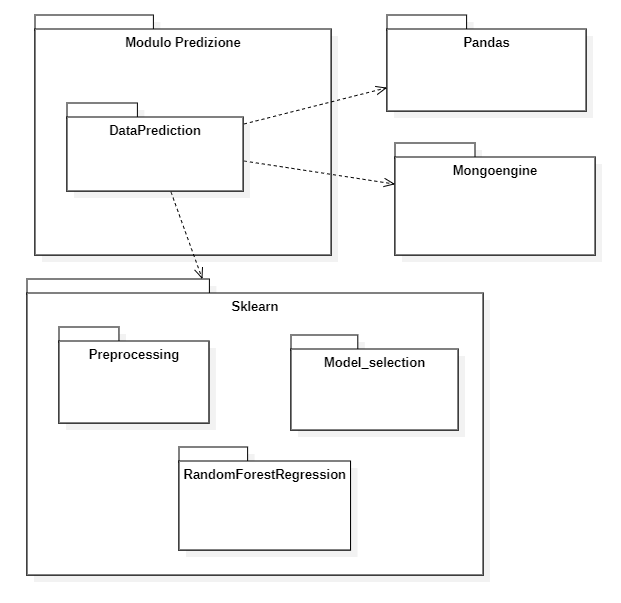
\includegraphics{../immagini/diag_PB/diag_pack_pred.png}
		\caption{Diagramma dei package del modulo della predizione}
	\end{figure}
\end{center}

\section{Architettura Web-App}\label{ArchitetturaDelProdottoWebApp}
Per il modulo relativo al front-end$_G$, si è deciso di utilizzare il pattern \textit{Model-View-Controller}(MVC).
Questa scelta è dovuta al fatto che, essendo la web-app sviluppata con spring, il pattern è quello che più si adatta alla tipologia sia di modellazione sia di scopo.
Lo scambio di dati tra fron-end e back-end avviene attraverso il pattern architetturale REST. Si è deciso questo pattern per avere un oggetto di scambio tra le due parti unico strutturalmente e quindi non è essere vincolato dalla struttura presente nel database.
Questo permette di aumentare la portabilità dell'applicazione web potendo applicare il back-end, possibilmente, a diversi front-end. Le richieste che il front-end effettua al back-end sono HTTP Request GET, quindi sono sempre richieste di visione di informazioni per poi essere utilizzate per aggiornare la parte grafica visibile dal client.
%Inserire
%Grafici

	\chapter{Requisiti soddisfatti}
In questo capitolo vengono illustrati attraverso grafici a torta e tabelle i requisiti funzionali che sono stati implementati all'interno della demo sviluppata per la \textit{Revisione di qualifica}. Utilizzando la codifica descritta all'interno delle \textit{Norme 3.0.0}

\section{Tabella requisiti funzionali}
\def\tabularxcolumn#1{m{#1}}
{\rowcolors{2}{RawSienna!90!RawSienna!20}{RawSienna!70!RawSienna!40}

	\begin{center}
		\renewcommand{\arraystretch}{1.4}
		\begin{longtable}{|p{4cm}|p{4cm}|}
			\hline
			\rowcolor{airforceblue}
			\makecell[c]{\textbf{Codice Requisito}} & \makecell[c]{\textbf{Soddisfatto}} \\
			%fase 1
			\hline
			\centering RSFO1  & \makecell[tc]{Soddisfatto} \\
			% \shortstack{Capitolato\\Verbale esterno 17-12-2020}   \\
			\hline
			\centering RSFF2 & \makecell[tc]{Non soddisfatto} \\
			\hline
			\centering RSFO3 & \makecell[tc]{Soddisfatto}  \\
			\hline
			\centering RSFO4 & \makecell[tc]{Soddisfatto}  \\
			\hline
			\centering RSFO4.1 & \makecell[tc]{Soddisfatto}  \\
			\hline
			\centering RSFO4.2  & \makecell[tc]{Soddisfatto}  \\
			%fase 2
			\hline
			\centering RSFO5 & \makecell[tc]{Soddisfatto}  \\
			\hline
			\centering RSFD5.1 & \makecell[tc]{Non soddisfatto}  \\
			\hline
			\centering RSFD6 & \makecell[tc]{Non soddisfatto}  \\
			%fase 3
			\hline
			\centering RSFO7 & \makecell[tc]{Soddisfatto}  \\
			\hline
			\centering RSFO8  &  \makecell[tc]{Soddisfatto} 	\\
			\hline
			\centering RSFO9 &  \makecell[tc]{Soddisfatto} 	\\
			\hline
			\centering RSFO10 &  \makecell[tc]{Soddisfatto} 	\\
			\hline
			\centering RSFO11 &  \makecell[tc]{Soddisfatto} 	\\
			\hline
			\centering RSFF12  &  \makecell[tc]{Non soddisfatto} 	\\
			\hline
			\centering RSFD13 &  \makecell[tc]{Non soddisfatto} 	\\
			\hline
			\centering RSFD14  &  \makecell[tc]{Non soddisfatto} 	\\
			\hline
			\centering RSFF15 &  \makecell[tc]{Non soddisfatto} 	\\
			\hline
			\centering RSFF16 &  \makecell[tc]{Non soddisfatto} 	\\
			\hline
			\centering RSFO17 & \makecell[tc]{Soddisfatto} \\
			\hline
			\centering RSFO18 &  \makecell[tc]{Soddisfatto} \\
			\hline
			\centering RSFO18.1 & \makecell[tc]{Soddisfatto} \\
			\hline
			\centering RSFO19 & \makecell[tc]{Soddisfatto} \\
			\hline
			\centering RSFO20 & \makecell[tc]{Soddisfatto} \\
			\hline
			\centering RSFO21 & \makecell[tc]{Soddisfatto} \\
			\hline
			\centering RSFO22  & \makecell[tc]{Soddisfatto} \\
			\hline
			\centering RSFO22.1  & \makecell[tc]{Soddisfatto} \\
			\hline
			\centering RSFO22.2  & \makecell[tc]{Soddisfatto} \\
			\hline
			\centering RSFF23 & \makecell[tc]{Soddisfatto} \\
			\hline
			\centering RSFO24 & \makecell[tc]{Soddisfatto} \\
			\hline
			\centering RSFO25 & \makecell[tc]{Soddisfatto} \\
			\hline
			\centering RSFO26 & \makecell[tc]{Soddisfatto} \\
			\hline
			\centering RSFO27 & \makecell[tc]{Soddisfatto} \\
			\hline
			\centering RSFO28 & \makecell[tc]{Soddisfatto} \\
			\hline
			\centering RSFD29 & \makecell[tc]{Non soddisfatto} \\
			\hline
			\centering RSFO30 & \makecell[tc]{Soddisfatto} \\
			\hline
			\centering RSFF31 & \makecell[tc]{Non soddisfatto} \\
			\hline
			\centering RSFO32 & \makecell[tc]{Soddisfatto} \\
			\hline
			\centering RSFO32.1 & \makecell[tc]{Soddisfatto} \\
			\hline
			\centering RSFO32.1.1 & \makecell[tc]{Soddisfatto} \\
			\hline
			\centering RSFO32.1.2 & \makecell[tc]{Soddisfatto} \\
			\hline
			\centering RSFO32.1.3 & \makecell[tc]{Soddisfatto} \\
			\hline
			\centering RSFO32.2 & \makecell[tc]{Soddisfatto} \\
			\hline
			\centering RSFD33 & \makecell[tc]{Non soddisfatto} \\
			\hline
			\centering RSFD33.1 & \makecell[tc]{Soddisfatto} \\
			\hline
			\centering RSFD33.2 & \makecell[tc]{Non soddisfatto} \\
			\hline
			\centering RSFD34 & \makecell[tc]{Non soddisfatto} \\
			\hline
			\centering RSFD35 & \makecell[tc]{Non soddisfatto} \\
			\hline
			\centering RSFD36 & \makecell[tc]{Non soddisfatto} \\
			\hline
			\centering RSFD36.1 & \makecell[tc]{Non soddisfatto} \\
			\hline
			\centering RSFD36.2 & \makecell[tc]{Non soddisfatto} \\
			\hline
			\centering RSFD37 & \makecell[tc]{Non soddisfatto} \\
			\hline
			\centering RSFD37.1 & \makecell[tc]{Non soddisfatto} \\
			\hline
			\centering RSFD38 & \makecell[tc]{Non soddisfatto} \\
			\hline
			\centering RSFD39 & \makecell[tc]{Non soddisfatto} \\
			\hline
			\centering RSFD40 & \makecell[tc]{Non soddisfatto} \\
			\hline
			\centering RSFD41 & \makecell[tc]{Soddisfatto} \\
			\hline
			\rowcolor{white}
			\caption[Tabella requisiti funzionali]{Requisiti funzionali soddisfatti}\label{3.1}\\
		\end{longtable}%\captionof{table}{Requisiti funzionali}
\end{center}
\section{Grafici requisiti funzionali}\label{GraficiRequisitiFunzionali}
Nel grafico seguente vengono visualizzati tutti i requisiti funzionali soddisfatti.
\begin{center}
	\begin{figure}[H]
		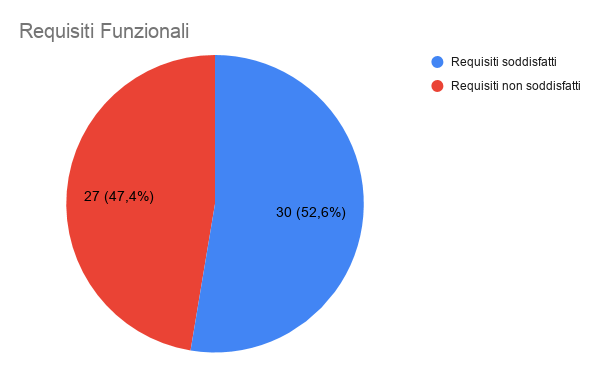
\includegraphics[scale=0.8]{../immagini/diag_PB/torta_RSF.png}
		\caption{Diagramma a torta di tutti i requisiti funzionali soddisfatti}
	\end{figure}
\end{center}

Nel grafico seguente vengono visualizzati tutti i requisiti funzionali obbligatori soddisfatti.

\begin{center}
	\begin{figure}[H]
		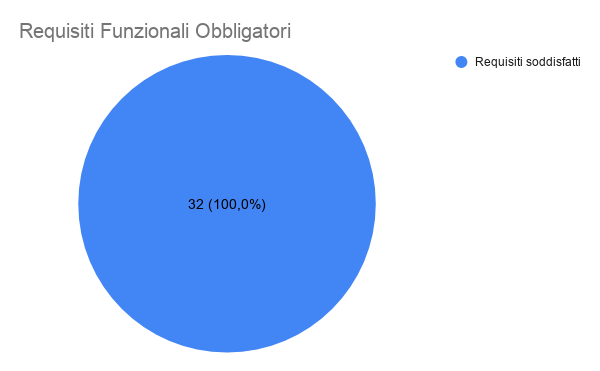
\includegraphics[scale=0.8]{../immagini/diag_PB/torta_RSFO.png}
		\caption{Diagramma a torta di tutti i requisiti funzionali obbligatori soddisfatti}
	\end{figure}
\end{center}

	% bibliography, glossary and index would go here.
	
\end{document}